\subsection{Three models of a slow device}
\label{sec:models}

Figure~\ref{fig:models} runs the code the fork benchmarked, its thread engine over
1{,}000 traced files plus the plain sequential loop its results file calls
``sequential'', under the three slow-device models of \S\ref{sec:method}, with a
5\,ms delay. Table~\ref{tab:models} gives the 1\,ms and 10\,ms cases.

\begin{figure*}[t]
\centering
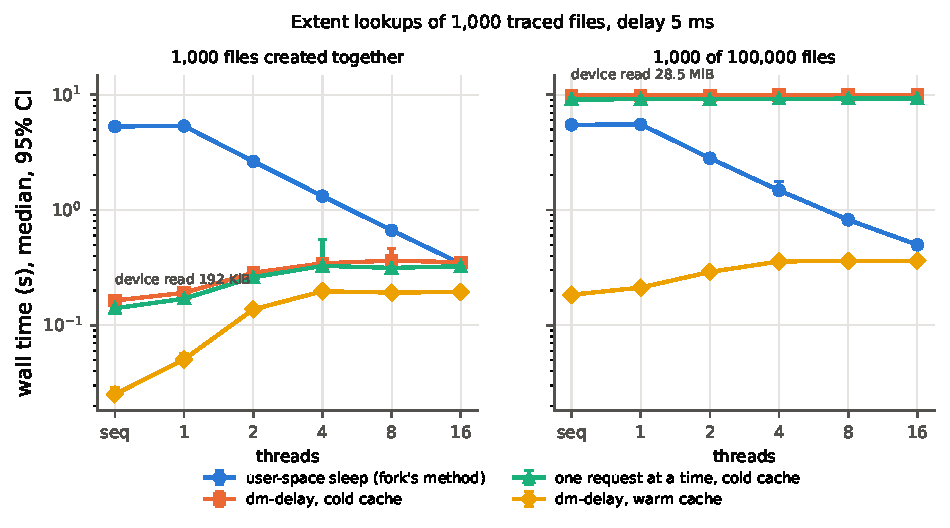
\includegraphics[width=0.9\textwidth]{../figs/e5_models_d5.pdf}
\caption{Wall time of the fork's extent-lookup engine against threads (``seq'': the
plain sequential loop) for 1{,}000 traced files, with a 5\,ms delay injected three
ways. Left: 1{,}000 files of 100\,KB created together; right: 1{,}000 files sampled
from a tree of 100{,}000. Medians of five runs with 95\% bootstrap intervals; the
labels give the data the device actually read in a cold run.}
\label{fig:models}
\end{figure*}

\paragraph{The user-space model reproduces the published speedup.} With
\texttt{time.sleep(0.005)} before every lookup, the sequential loop takes 5.31\,s and
16 threads take 0.343\,s, a speedup of 15.5$\times$ (95\% CI 14.3--15.7), close to the
fork's 12.74$\times$ (its sequential time, 7.28\,s, suggests a coarser sleep on that
machine). The model's prediction does not depend on the files at all: the scattered
case gives 11.0$\times$.

\paragraph{With the delay at the block layer, there is nothing to overlap.} When the
same 5\,ms is added to every read that reaches the device, the 1{,}000 files created
together are looked up in 0.164\,s from a cold cache by the sequential loop, 32 times
faster than the user-space model predicts, because the whole job reads only 192\,KiB
from the device: the directory blocks and a few inode-table blocks, each of which
holds the inodes of 16 files and is read ahead in groups of 32 blocks
(\texttt{inode\_readahead\_blks}, 32 on our kernel~\cite{kernelext4admin}), so one
miss brings in the inodes of 512 files.
Threads only add overhead (16 threads: 0.352\,s, 0.47$\times$). With a warm cache the
device is not touched at all and the sequential loop takes 25\,ms.

\paragraph{Scattered metadata is slow, but not in a way threads can fix.} When the
1{,}000 traced files are spread over a tree of 100{,}000, a cold run reads 28.5\,MiB
and takes 9.82\,s; but 16 threads take 9.99\,s, under dm-delay, which lets any number of
requests wait at once, and under the one-request-at-a-time device alike. Almost all of
the device time is spent before the threads start, in the single walk that builds the
inode map (\S\ref{sec:decompose}).

\begin{table}[t]
\caption{Speedup of 16 threads over the sequential loop (median, 95\% CI), and the
sequential loop's time, for each delay model. Five runs each.}
\label{tab:models}
\small
\input{../results/tab_models.tex}
\end{table}
